\chapter[Otimização bio-inspirada]{Otimização bio-inspirada}

Grande parte dos problemas de otimização envolvem encontrar a melhor opção num conjunto de possibilidades que cresce de maneira exponencial \cite{Viggo1992}. Tais problemas são impossíveis de serem resolvidos de modo satisfatório com a tecnologia atual e necessitam de estratégias inteligentes para se aproximarem da solução ótima em tempo hábil. Dentre essas estratégias, destacam-se os algoritmos gulosos e os algoritmos de busca bio-inspirados.

Os algoritmos gulosos \cite{GreedyAlgorithms} são estratégias relativamente simples que, apesar de nem sempre obterem a solução ótima, normalmente aproximam-se bem dela. Tais métodos são geralmente utilizados quando apenas um critério é envolvido na otimização. Quando mais de um objetivo deve ser analisado, o problema fica bem mais complexo e essa abordagem deixa de ser indicada.

A otimização bio-inspirada \cite{BioInspiredOptimization} lança mão de estratégias baseadas na natureza para se encontrar boas soluções de forma eficiente. Assim como os algoritmos gulosos, não é garantida a obtenção da solução ótima, mas com uma boa modelagem do problema, é possível encontrar soluções suficientemente próximas. Na natureza, o processo de obter uma boa solução é usado a todo momento, desde a forma como as espécies evoluem, até a maneira como uma simples formiga encontra o caminho mais curto entre a colônia e uma fonte de comida. Ao observar processos comuns da natureza, estudiosos encontraram maneiras simples e eficientes de se resolver diversos problemas de otimização. Os principais métodos de otimização bio-inspirados na literatura são os algoritmos evolutivos e os algoritmos de inteligência coletiva (\textit{swarm intelligence}). Dentre os evolutivos, destacam-se os algoritmos genéticos (AGs), e dentre os coletivos, destacam-se as colônias de formigas (ACOs) e os enxames de partículas (PSOs).

Os algoritmos genéticos se inspiram na teoria da evolução de Darwin \cite{Darwin1859}. Na evolução das espécies, cada indivíduo possui um material genético que é cruzado com os genes de outro representante da espécie para gerar um novo indivíduo. Durante tal cruzamento, alguns indivíduos sofrem mutações aleatórias que podem alterar parte de sua carga genética e, com isso, suas características (fenótipo). O ambiente determina a parte da população que sobrevive e a parte que perece. Os indivíduos sobreviventes, ou seja, aqueles bem adaptados ao ambiente, possuem maiores chances de se reproduzir e espalhar suas boas características genéticas. Desta forma, a evolução das espécies nada mais é que um processo otimizador, no qual indivíduos são gerados e os melhores são selecionados. Esse processo é repetido ao longo das gerações, até que se obtenha indivíduos bem adaptados ao ambiente em questão.

Os ACOs são inspirados no comportamento das formigas, organismos simples que quando analisados em conjunto (colônia) apresentam comportamento complexo \cite{Dorigo1996}. O interesse nas formigas vem da observação de que, ao buscarem por comida, acabam por encontrar o caminho mais rápido entre a fonte de alimento e o formigueiro. Como podem seres tão simples resolverem eficientemente um problema de otimização? Estudos revelaram que as formigas se baseiam no depósito de feromônios para se guiarem. Quanto mais forte o feromônio em um caminho, maior as chances dele ser utilizado pelas formigas. Tal comportamento serviu de inspiração para os algoritmos de otimização bio-inspirados, dando origem ao \ac{ACO}.

Os algoritmos baseados em enxames de partículas (PSOs), assim como os ACOs são inspirados no comportamento emergente de populações de animais simples. Os PSOs se inspira na navegação de pássaros, onde cada elemento da formação se guia através dos pássaros à frente. O algoritmo se baseia na direção e velocidade de cada elemento do enxame, determinando a exploração do espaço de busca através de operações vetoriais. Portanto, é uma estratégia indicada para problemas contínuos, não sendo indicada para os problemas explorados nesta dissertação (embora existam exemplos de discretização dos PSOs na literatura).

Em geral, todo algoritmo de otimização bio-inspirado inicia sua busca por meio da geração aleatória de soluções. Após essa geração inicial, inicia-se uma etapa recorrente, na qual as melhores soluções guiam a construção de novas soluções que serão submetidas ao mesmo processo até que uma condição de parada seja atingida. Como não é necessário gerar todas as soluções possíveis, são métodos eficazes que, quando bem modelados, encontram um conjunto de boas soluções que resolvem o problema. Uma das principais diferenças entre os algoritmos bio-inspirados e as demais estratégias de otimização é o fato de que os primeiros produzem um conjunto de soluções aproximadas até o último passo do processo, quando, retorna a solução melhor avaliada. Essa é uma característica interessante para a otimização multiobjetivo, pois nela poder-se-ia retornar todas as soluções não-dominadas ao invés de apenas uma.

\section{Algoritmos Genéticos}
\label{section_ag}
Os algoritmos genéticos (AGs) são métodos de busca baseados na teoria da evolução de Charles Darwin \cite{Darwin1859}. A teoria de Darwin, hoje já endossada por diversas observações no campo da biologia, parte do princípio de que os organismos se adaptam ao ambiente em que vivem através de seleção natural, cruzamento e mutação. Mudanças nos genes (genótipo) de um indivíduo da população afetam suas características genéticas (fenótipo) e podem ajudá-lo a sobreviver em seu habitat ou atrapalhá-lo. Os indivíduos com características favoráveis têm maiores chances de sobreviver e reproduzir, passando essas características para a geração seguinte. Dessa forma, ao longo de milhões de anos, organismos simples se tornam complexos e extremamente adaptados ao meio.

A ideia dos algoritmos genéticos é aplicar o mesmo conceito da evolução natural na computação. O algoritmo parte de um conjunto de soluções aleatórias (população inicial) e, após várias iterações de seleção, cruzamento (ou \textit{crossover}) e mutação, obtém um conjunto de soluções (população final) que espera-se que resolvam bem o problema. Nesse processo, o indivíduo na população representa uma solução, o meio representa o problema e as operações de cruzamento e mutação devem ser definidas, respectivamente, de forma a permitir a combinação de duas soluções e uma alteração aleatória em uma solução. A seleção dos pais e a sobrevivência dos mais aptos representam a metáfora da seleção natural. 
\\
Conforme ilustrado na \autoref{fig_flux_ga}, o funcionamento básico de um AG inicia-se com a geração da população inicial. Nessa etapa, os indivíduos da população são normalmente gerados de forma aleatória e, em seguida, avaliados quanto à sua aptidão ao meio. No caso de um problema de otimização para uma função objetivo $f$, a aptidão de um indivíduo $x$ é dada por $f(x)$. Após esse processo de inicialização, parte-se para a evolução das gerações que consiste na repetição das seguintes etapas:

\begin{figure}[!htbp]
	\centering
	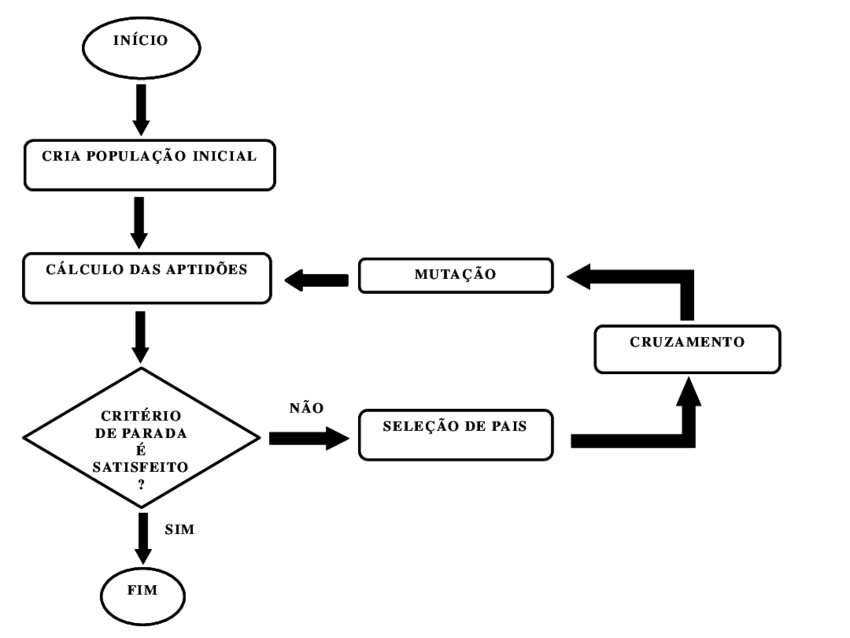
\includegraphics[width=1\textwidth]{cap_otimizacao-bio/figs/ga-flux.png}
	\caption{\label{fig_flux_ga}Fluxograma de um AG. Retirado de \cite{FiguraGA}}
\end{figure}

\begin{enumerate}  
	\item Sortear os pares de pais; 
	\item Aplicar o cruzamento em cada par e gerar os filhos; 
	\item Aplicar a mutação aos filhos, de acordo com uma taxa de mutação pré-estabelecida;
	\item Avaliar os filhos;
	\item Selecionar entre pais e filhos quais indivíduos formarão a população da iteração seguinte (reinserção).
\end{enumerate}

A evolução das gerações do AG termina quando uma condição de término estabelecida pelo usuário é atingida, por exemplo, encontrar a solução ótima do problema (quando conhecida) ou atingir um número máximo de gerações. Cada etapa de execução do AG é descrita com mais detalhes a seguir.

\subsection{Representação do indivíduo}
A principal dificuldade ao se elaborar um algoritmo genético é definir a representação do indivíduo. Cada indivíduo representa uma possível solução para o problema investigado e deve ser codificado em uma estrutura que possibilite e/ou favoreça a realização das operações genéticas de mutação e cruzamento. Na proposição original do AG \cite{Goldberg1989}, o indivíduo é representado de forma binária, ou seja, a solução para o problema é codificada em uma cadeia de bits, na qual cada posição pode facilmente ser invertida (mutação) ou copiada de um cromossomo para outro (cruzamento).

No problema da mochila 0/1, por exemplo, existe um conjunto de itens $I$ com pesos e valores e uma mochila com capacidade limitada. Deve-se descobrir qual a melhor forma de se arranjar os itens de maneira que a soma dos valores de cada um seja máxima e que a capacidade da mochila não seja excedida. Para representar uma solução deste problema em um AG, basta assumir um vetor binário de tamanho igual a $|I|$, onde diz-se que o item está na mochila se sua posição correspondente no vetor binário é 1 e não está, caso contrário.

Outras representações de indivíduos também são possíveis, mas apresentam novos desafios. Por exemplo, em problemas de menores caminhos, normalmente trabalha-se com árvores e caminhos. No PRM, o indivíduo é uma árvore e tanto a mutação quanto o cruzamento devem ser operações em árvores.

Para elaborar a representação do indivíduo no AG, deve-se levar em consideração a facilidade de manipulação da estrutura, a possibilidade de se introduzir um fator aleatório (mutação) e, principalmente, a representação das características de ambos os pais nos filhos. Se a estrutura não permite a herança de características, não é uma boa escolha para se utilizar em um algoritmo genético. Além disso, é preciso garantir a unicidade da forma de representação, ou seja, cada solução pode ser representada de uma única maneira e cada indivíduo deve representar uma única solução (relação um-para-um).

\subsection{Seleção de pais}
A estratégia para selecionar os pais que contribuirão para a composição genética da geração seguinte do AG deve ser escolhida de acordo com o propósito do algoritmo. Dependendo do problema, pode ser mais desejável uma convergência rápida que uma exploração mais profunda do espaço de busca, por exemplo. Os três métodos abaixo estão entre os mais empregados na etapa de seleção.

\begin{enumerate}
	\item Seleção elitista: os $t_e\%$ indivíduos da população com melhor aptidão formam um grupo de onde se sorteiam todos os pares de pais necessários para gerar a população de filhos. $t_e$ representa a taxa de elitismo, que é um parâmetro do AG. Dessa forma, não há chance de indivíduos muito ruins propagarem suas características. Portanto, a população converge para indivíduos iguais (ou muito parecidos) rapidamente, sem explorar partes do espaço de busca aparentemente ruins. Isso pode prejudicar o algoritmo em problemas com muitos mínimos locais, onde o fato de existir uma solução ruim não quer dizer que as soluções próximas também o são.
	\item Roleta: é um método menos rigoroso que o anterior. Cada indivíduo recebe uma probabilidade de ser selecionado de acordo com sua aptidão. Os indivíduos com maior aptidão receberão probabilidade alta e dificilmente não serão selecionados, enquanto indivíduos muito ruins raramente se tornarão pais. Apesar disso, toda solução tem chance de ser escolhida, o que melhora a exploração do espaço de busca em relação a estratégia anterior, mas pode diminuir a velocidade de convergência. Esta estratégia é um meio-termo entre a seleção elitista e a seleção por torneio, explicada a seguir.
	\item Seleção por torneio: esta é a estratégia com a menor pressão seletiva dentre os três métodos, ou seja, aquele que dá a maior chance aos indivíduos ruins de se tornarem pais e propagarem suas características. O torneio consiste em selecionar dois indivíduos aleatoriamente e escolher como primeiro pai aquele com a melhor aptidão, da mesma forma, sorteia-se dois outros indivíduos na população, diferentes do primeiro pai, e define-se como segundo pai a solução com melhor aptidão. O torneio básico é o torneio de dois, mas para aumentar a pressão seletiva, é possível realizar o torneio com um maior número de representantes da população. Dentre as três estratégias, esta é a que melhor explora o espaço de busca. Por outro lado, é possível que, ao explorar demasiadamente o espaço, o AG não consiga convergir.
\end{enumerate}

\subsection{Operadores genéticos}
Nos algoritmos genéticos, destacam-se duas operações principais que atuam sobre o código do indivíduo: cruzamento e mutação. O cruzamento e a mutação estão diretamente ligados com a forma de representação do indivíduo.

Num algoritmo genético, cada iteração do laço principal é chamada de geração. No início de cada geração, sorteia-se pares de pais de acordo com suas aptidões para que seja gerada uma nova população de filhos. A quantidade de pares de pais sorteados é determinada pela taxa de crossover, a qual é um parâmetro de configuração do AG. Cada par é composto de duas cadeias genéticas (cromossomos), uma correspondente a cada indivíduo do par. Para gerar o filho, cruza-se os dois cromossomos a fim de se obter dois novos indivíduos que compartilhem características de ambos genitores. Esse processo é conhecido como cruzamento, ou \textit{crossover}. Existem várias maneiras de se cruzar cadeias genéticas. A escolha depende principalmente da estrutura de dados usada para representar o cromossomo. A estrutura mais comum é a cadeia binária \cite{Goldberg1989}, onde uma solução é codificada em uma cadeia de 0's e 1's. Nesse caso, a forma mais simples de efetuar o cruzamento é gerar duas novas cadeias de bits (filhos), onde parte do material genético (posições na cadeia) pertence a um pai e o restante do material é proveniente do outro. Os filhos gerados em um cruzamento adotam materiais genéticos complementares de cada pai. Por exemplo, se o filho 1 herda os n primeiros genes do pai 1 e o restante do pai 2, o filho 2 herdará os $n$ primeiros genes do pai 2 e o restante do pai 1. A \autoref{fig_cross_ponto_unico} ilustra este tipo de cruzamento. Existem diversas formas de se combinar duas cadeias de bits, dentre elas podem-se destacar:

\begin{itemize}  
	\item Ponto de cruzamento único: uma posição $i$ de uma das cadeias é sorteada. O filho 1 herda os $i$ primeiros genes do pai 1 e restante do pai 2, enquanto que o filho 2 adota o material genético complementar. Na \autoref{fig_cross_ponto_unico}, é ilustrado um exemplo onde o ponto de cruzamento é estabelecido na metade.
	\item Dois pontos de cruzamento: ao invés de se utilizar apenas um ponto para dividir o material genético, este método divide a cadeia binária em três partes. Nesse caso, um filho herda a primeira e terceira partes de um pai e a segunda do outro.
	\item Cruzamento uniforme: cada bit do filho é obtido de forma aleatória, pode vir tanto do pai 1 quanto do pai 2. Em termos de implementação, sorteia-se uma máscara binária e para cada bit 0 da máscara, copia-se o gene do pai 1 para o filho. Para cada bit 1, copia-se o gene do pai 2.
	\item Cruzamento aritmético: realiza-se uma operação binária (ex: AND, OR, XOR, etc.) entre os cromossomos do pai 1 e do pai 2.
\end{itemize}

\begin{figure}[!htbp]
	\centering
	\renewcommand{\arraystretch}{2} 
	\begin{tabular}{rl}
		Pai 1: & 
		\renewcommand{\arraystretch}{1.15} 
		\begin{tabular}{|c|c|c|c|c|c|}
			\hline 
			\rowcolor[HTML]{F5D1CF}
			0 & 0 & 1 & 0 & 1 & 1 \\
			\hline 
		\end{tabular}
		\\
		Pai 2: & 
		\renewcommand{\arraystretch}{1.15} 
		\begin{tabular}{|c|c|c|c|c|c|}
			\hline 
			\rowcolor[HTML]{CCCCFF}
			1 & 0 & 0 & 1 & 1 & 0 \\
			\hline 
		\end{tabular}
		\\
		Filho 1: & 
		\renewcommand{\arraystretch}{1.15} 
		\begin{tabular}{|c|c|c|c|c|c|}
			\hline 
			\cellcolor[HTML]{F5D1CF}0 & \cellcolor[HTML]{F5D1CF}0 & \cellcolor[HTML]{F5D1CF}1 & \cellcolor[HTML]{CCCCFF}1 & \cellcolor[HTML]{CCCCFF}1 & \cellcolor[HTML]{CCCCFF}0 \\
			\hline 
		\end{tabular}
		\\
		Filho 2: & 
		\renewcommand{\arraystretch}{1.15} 
		\begin{tabular}{|c|c|c|c|c|c|}
			\hline 
			\cellcolor[HTML]{CCCCFF}1 & \cellcolor[HTML]{CCCCFF}0 & \cellcolor[HTML]{CCCCFF}0 & \cellcolor[HTML]{F5D1CF}0 & \cellcolor[HTML]{F5D1CF}1 & \cellcolor[HTML]{F5D1CF}1 \\
			\hline 
		\end{tabular}
	\end{tabular}
	\caption{\label{fig_cross_ponto_unico}Exemplo de \textit{crossover} com cruzamento de ponto único, onde o ponto de cruzamento está na metade do material genético.}
\end{figure}

A fim de melhorar a diversidade entre as soluções avaliadas, uma pertubação nos genes dos indivíduos é gerada durante a busca, possibilitando a exploração de elementos ausentes na população atual. Para isso, após gerar o cromossomo de cada filho, é preciso permitir que ocorra uma mutação, ou seja, uma mudança aleatória no material genético. A chance de uma mutação ocorrer depende de um parâmetro do AG chamado de ``taxa de mutação''. O processo de alteração genética aleatória depende da representação do indivíduo. No caso de uma cadeia binária, por exemplo, é simples, basta sortear um bit e invertê-lo. Em árvores, a mutação pode consistir na eliminação de algum vértice e na reconexão aleatória. Em grafos ponderados, alterar os pesos de uma aresta pode ser uma boa ideia. A definição do processo de mutação dependerá do problema e pode ser feita de várias maneiras diferentes, desde que produza uma pequena diferença no indivíduo e que ele continue representando uma solução válida.

O cruzamento normalmente gera um ou dois filhos para cada pai. Em todos os métodos descritos anteriormente é possível obter um segundo filho com o material genético não utilizado.

\subsection{Reinserção da População}
Independente do número de filhos gerados, após os processos de \textit{crossover} e mutação, a população será maior que o limite máximo permitido, exigindo a eliminação de alguns indivíduos (seleção natural). A reinserção opera sobre a aptidão (função de avaliação ou \textit{fitness}) de cada indivíduo da população. Diversas estratégias podem ser aplicadas nesse processo de seleção, também conhecido como reinserção. Por exemplo, a seleção natural sem elitismo, simplesmente elimina a população mais velha (pais). A seleção natural com elitismo mantém um percentual da população de pais (elite), completando-a com os melhores filhos. Outro tipo de elitismo é a seleção dos melhores indivíduos. Essa estratégia é normalmente mais interessante, pois permite a sobrevivência dos indivíduos mais aptos considerando a totalidade da população, sendo assim, avalia-se todos os pais e filhos e mantém-se aqueles com melhor aptidão.

\section{Otimização por Colônia de formigas}
\label{section_aco}
A otimização por colônia de formigas (ACO), proposto em \cite{Dorigo1996}, é um modelo de busca bio-inspirado que parte da ideia de que estruturas simples, com alguma espécie de comunicação, podem gerar um comportamento complexo quando operam em conjunto, de forma cooperativa. A inspiração do ACO é o forrageamento em uma colônia de formigas. Na natureza, observa-se que as formigas, mesmo sendo seres vivos simples, conseguem encontrar o melhor caminho entre o formigueiro e a fonte de comida. A partir do estudo desse comportamento, descobriu-se que tal faceta é possível através de uma comunicação indireta entre os animais. Ao fazer um caminho, as formigas depositam uma substância chamada feromônio, a qual pode ser percebida por outros membros da espécie. Uma formiga ao decidir qual caminho percorrer, tem maior chance de escolher aquele com a maior quantidade de feromônios. Além disso, a substância evapora com o tempo. Dessa forma, quanto menor o caminho, maior a frequência com a qual as formigas depositarão feromônio e, portanto, maior será a chance de ser escolhido.

Ao trazer o conceito de colônia de formigas para a computação, observa-se um grande potencial para se resolver problemas em grafo. Por exemplo, para descobrir o menor caminho entre os vértices $A$ e $B$ em um grafo não ponderado $G$, basta simular várias formigas que partem de $A$ e chegam em $B$, fazendo um caminho baseado na quantidade de feromônios das arestas. Ao final de cada iteração, atualiza-se o valor do feromônio em cada aresta de acordo com a evaporação e com as arestas percorridas pelas formigas. Dessa forma, espera-se que, após várias iterações, a quantidade de feromônios seja suficiente para guiar uma formiga pelo melhor caminho entre $A$ e $B$. O fluxograma de um ACO é mostrado na \autoref{fig_flux_aco}.

\begin{figure}[!htbp]
	\centering
	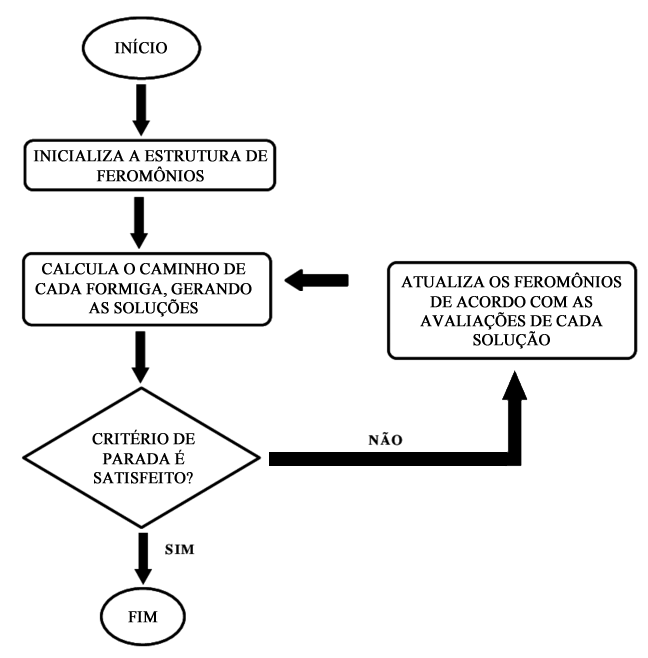
\includegraphics[width=0.7\textwidth]{cap_otimizacao-bio/figs/aco-flux.png}
	\caption{\label{fig_flux_aco}Fluxograma de um ACO.}
\end{figure}

O algoritmo inicia com a limpeza dos feromônios das arestas, ou seja, é atribuído zero para a quantidade de feromônio depositado em cada aresta do grafo. Após essa limpeza, inicia-se o processo iterativo do algoritmo onde, a cada iteração, as formigas na colônia percorrem o caminho do vértice de partida (formigueiro) ao nó destino (fonte de comida). Dependendo da formulação do problema, o caminho de volta também pode ser realizado. Ao final de cada iteração, atualiza-se os feromônios em cada aresta. O algoritmo termina quando uma condição de parada pré-determinada é atingida, normalmente um número máximo de iterações. As etapas principais da execução de um ACO são descritas a seguir.

\FloatBarrier
\subsection{Representação da solução}
No ACO, a solução é representada pelo caminho feito pela formiga no grafo, normalmente uma lista de vértices, uma árvore ou um subgrafo do grafo de entrada. Por exemplo, no problema de encontrar o menor caminho, a solução pode ser uma lista de vértices que representa o percurso desse caminho. Caso seja necessário encontrar caminhos entre a raiz e diversos destinos, pode-se representar a solução como uma árvore. Nem sempre é fácil decidir a codificação de uma solução. No problema da mochila, por exemplo, não é trivial a visualização de um grafo no processo da construção da solução. Nesse caso, uma possível representação é a associação de feromônios diretamente aos itens, através de um vetor de feromônios ao invés de uma matriz.

\subsection{Construção da solução} \label{section_construcao_solucao}
\label{section_otimizacao_aco_construcao}
Independentemente da representação escolhida, deve ser possível relacionar cada parte da solução com uma quantidade de feromônios na estrutura principal. Por exemplo, no caso de grafos, as arestas escolhidas para montar a solução devem ter seus feromônios incrementados a fim de guiar as próximas formigas. Em cada época (iteração do algoritmo) um número pré-determinado de soluções é construído, onde cada formiga decide quais partes serão adotadas em sua solução, com base nos respectivos valores de feromônios.

Além dos feromônios, as formigas ainda utilizam as informações de heurística para decidir o próximo passo. Uma heurística é uma função que estima a qualidade do caminho e normalmente representa o peso de uma aresta. Estando em um vértice $i$ de um grafo $G$, uma formiga tem probabilidade $p(i,j)$ de escolher a aresta que leva ao vértice adjacente $j$. Essa probabilidade é calculada pela seguinte equação:

\[ p(i,j) = \frac{\tau_{i,j}^\alpha * \eta_{i,j}^\beta}{\sum_{v \in adj(i)} \tau_{i,v}^\alpha * \eta_{i,v}^\beta} \]

Sendo:

\begin{itemize}  
	\item $\tau_{i,j}^\alpha$: feromônio na aresta $(i,j)$ elevado à constante $\alpha$, que representa a importância atribuída ao valor do feromônio. Representa o conhecimento sobre o ambiente (busca global).
	\item $\eta_{i,j}^\beta$: heurística da aresta $(i,j)$ elevada à constante $\beta$, que representa a importância atribuída à heurística. A heurística de uma aresta é dada em função do peso, como, por exemplo, $1/peso$, normalmente usado em problemas de minimização. Representa a visibilidade da formiga (busca local).
	\item $adj(i)$: são todos os vértices adjacentes a $i$, ou seja, todo vértice em $G$ para o qual é possível construir um caminho a partir de $i$ com apenas uma aresta.
\end{itemize}

O número de iterações (épocas), a quantidade de soluções geradas por iteração e as constantes alfa e beta são parâmetros de configuração de um algoritmo ACO. De forma geral, dado um grafo $G$ e um nó inicial, o processo de construção da solução sempre verifica todos os movimentos possíveis para a formiga, tomando sua decisão de acordo com os feromônios e as heurísticas de cada uma das possibilidades.

\subsection{Atualização dos feromônios}
Existem duas ocasiões onde o feromônio de uma aresta pode ser atualizado: no momento em que a formiga passa pela aresta e no fim de cada iteração. A maioria das implementações considera apenas o segundo caso, pois assim, é possível avaliar as soluções e incrementar os feromônios de acordo com os desempenhos obtidos. Ao fim de cada época, a quantidade de feromônio existente na aresta que liga os vértices i e j ($\tau_{i,j}$) é atualizada por:

\[ \tau_{i,j} = (1 - \rho) * \tau_{i,j} + \sum_{k \in formigas} \Delta\tau_{i,j}(k)\]

Sendo:

\begin{itemize}  
	\item $\rho$: parâmetro de configuração do ACO que corresponde ao coeficiente de evaporação. Determina o quão rápido o feromônio deve desaparecer das arestas após depositado.
	\item $formigas$: conjunto de todas as formigas na iteração.
	\item $\Delta\tau_{i,j}(k)$: quantidade de feromônio depositada pela formiga $k$ na aresta entre os vértices $i$ e $j$.
\end{itemize}

A quantidade de feromônio depositada por uma formiga $k$ em uma aresta entre os vértices $i$ e $j$ é dada por:

\[ \Delta\tau_{i,j}(k) = \begin{cases} \frac{Q}{L_k},& \text{se } x\geq 1\\ 0,& \text{caso contrário} \end{cases} \]

Sendo:

\begin{itemize}  
	\item $Q$: Quantidade máxima de feromônio que pode ser depositada por uma formiga.
	\item $L_k$: Custo da solução gerada pela formiga  $k$.
\end{itemize}

Considerando essas características, nossa pesquisa propõe uma nova versão de ACO para tratar problemas discretos com enfoque em otimização multiobjetivo.
